\documentclass{article}
\usepackage[utf8]{inputenc}
\usepackage{listings}
\usepackage[french]{babel}
\usepackage{graphicx}
\usepackage{pifont}
\usepackage{xcolor}
\usepackage[left=2.5cm,right=2.5cm,top=3cm,bottom=3cm]{geometry}
\renewcommand{\baselinestretch}{1.3}

\definecolor{deepblue}{rgb}{0,0,0.5}
\definecolor{deepred}{rgb}{0.6,0,0}
\definecolor{deepgreen}{rgb}{0,0.5,0}

% Default fixed font does not support bold face
\DeclareFixedFont{\ttb}{T1}{txtt}{bx}{n}{12} % for bold
\DeclareFixedFont{\ttm}{T1}{txtt}{m}{n}{12}  % for normal

\newcommand\pythonstyle{\lstset{
  language=Python,
  backgroundcolor=\color{white}, 
  basicstyle=\ttm\small,
  %otherkeywords={self},            
  %keywordstyle=\ttb\color{deepblue},
  emph={MyClass,__init__},          
  emphstyle=\ttb\color{deepred},    
  %stringstyle=\color{deepgreen},
  commentstyle=\color{red}, 
  frame=tb,                         
  showstringspaces=false,
  inputencoding=utf8,
  extendedchars=true,
  literate={é}{{\'e}}1 {î}{{\^i}}1 {ê}{{\^e}}1 {è}{{\`e}}1 {à}{{\`a}}1
}}
 
\lstset{literate=
  {á}{{\'a}}1 {é}{{\'e}}1 {í}{{\'i}}1 {ó}{{\'o}}1 {ú}{{\'u}}1
  {Á}{{\'A}}1 {É}{{\'E}}1 {Í}{{\'I}}1 {Ó}{{\'O}}1 {Ú}{{\'U}}1
  {à}{{\`a}}1 {è}{{\`e}}1 {ì}{{\`i}}1 {ò}{{\`o}}1 {ù}{{\`u}}1
  {À}{{\`A}}1 {È}{{\'E}}1 {Ì}{{\`I}}1 {Ò}{{\`O}}1 {Ù}{{\`U}}1
  {ä}{{\"a}}1 {ë}{{\"e}}1 {ï}{{\"i}}1 {ö}{{\"o}}1 {ü}{{\"u}}1
  {Ä}{{\"A}}1 {Ë}{{\"E}}1 {Ï}{{\"I}}1 {Ö}{{\"O}}1 {Ü}{{\"U}}1
  {â}{{\^a}}1 {ê}{{\^e}}1 {î}{{\^i}}1 {ô}{{\^o}}1 {û}{{\^u}}1
  {Â}{{\^A}}1 {Ê}{{\^E}}1 {Î}{{\^I}}1 {Ô}{{\^O}}1 {Û}{{\^U}}1
  {œ}{{\oe}}1 {Œ}{{\OE}}1 {æ}{{\ae}}1 {Æ}{{\AE}}1 {ß}{{\ss}}1
  {ű}{{\H{u}}}1 {Ű}{{\H{U}}}1 {ő}{{\H{o}}}1 {Ő}{{\H{O}}}1
  {ç}{{\c c}}1 {Ç}{{\c C}}1 {ø}{{\o}}1 {å}{{\r a}}1 {Å}{{\r A}}1
  {€}{{\euro}}1 {£}{{\pounds}}1 {«}{{\guillemotleft}}1
  {»}{{\guillemotright}}1 {ñ}{{\~n}}1 {Ñ}{{\~N}}1 {¿}{{?`}}1
}

\author{Alexis Lanoix et Jofrey Luc}
\title{Rapport init recherche}
\date{02/05/2017}

\begin{document}

\tableofcontents
\newpage

\newcommand\pythonexternal[2][]{{
\pythonstyle
\lstinputlisting[#1]{#2}}}

\section{Introduction et problématique}

Aujourd'hui, on dispose de moyens assez efficaces pour transformer automatiquement un texte prononcé dans un fichier audio en sa transcription écrite (par exemple, l'outil de sous-titrage automatique de Youtube). Le problème avec ces outils est qu'ils nécessitent toujours de savoir en quelle langue le texte est prononcé pour pouvoir le transcrire efficacement.\\
En effet, pour faire de la reconnaissance de la parole, il est essentiel de connaître le langage à traduire au préalable car il faut pouvoir utiliser les éléments propres à celui-ci.\\

\begin{figure}[h]
  \centerline{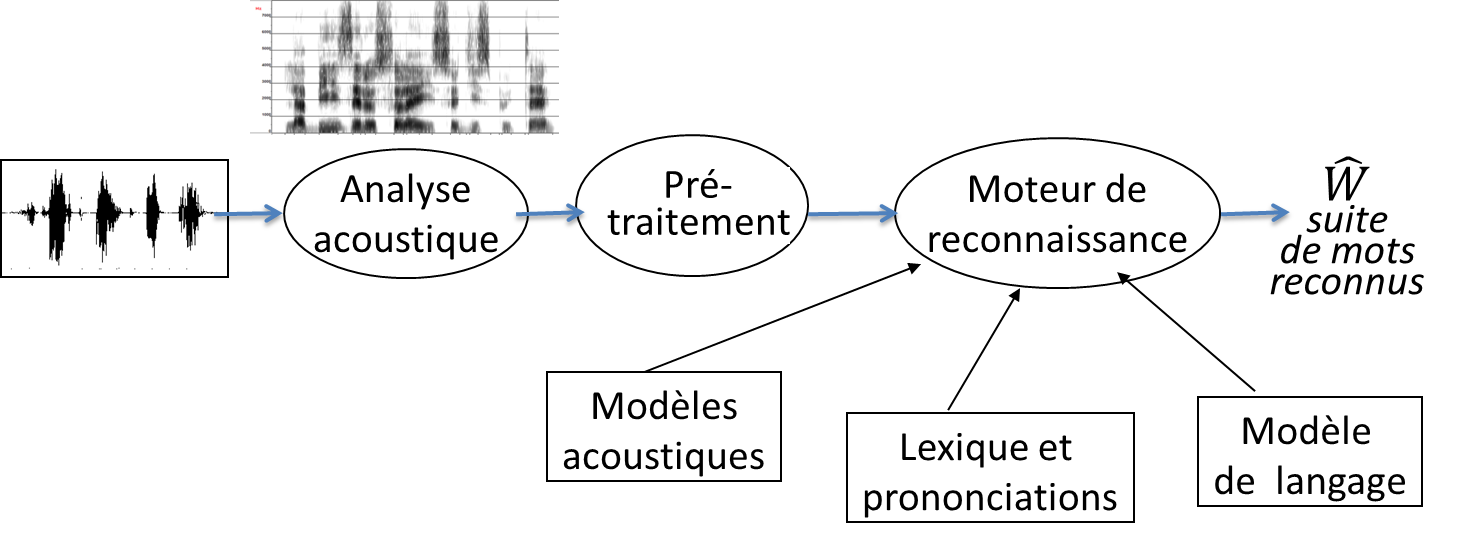
\includegraphics[scale=0.6]{img/schema_reco.png}}
  \caption{Schéma d'un système classique de reconnaissance de la parole}
\end{figure}

\noindent Ici, les éléments qui vont changer d'un langage à l'autre sont les modèles acoustiques, le lexique et les prononciations et le modèle de langage.\\
 \\
L'objectif de ce projet d'initiation à la recherche est donc de parvenir à détecter automatiquement la langue parlée dans un fichier audio. Cette détection automatique pourrait permettre de directement transcrire la parole prononcée dans le fichier, en utilisant la "bibliothèque" vocale correspondant à la langue parlée.\\
 \\
Pour ce faire, on utilisera des méthodes d'apprentissage automatique (machine learning) basées sur des réseaux de neurones profonds.
Dans un premier temps, le but sera de construire un réseau de neurones capable de déterminer, pour un fichier de parole homogène (même langue dans le fichier) donné en entrée, s'il s'agit de parole  allemande, anglaise, arabe ou française.\\
Ensuite, selon les performances du réseau précédent, nous tenterons de créer un système capable de détecter la langue d'un contenu audio de manière dynamique. Ainsi, nous pourrions repérer automatiquement, par exemple, une citation prononcée en anglais dans un flux de parole globalement allemande, pour pouvoir ainsi faciliter la transcription automatique d'un tel texte.

\section{Présentation générale}

\subsection{Les réseaux de neurones artificiels}

Les réseaux de neurones artificiels sont des modèles mathématiques qui sont souvent utilisés dans le domaine de l'apprentissage automatique, en tant qu'outils permettant de faire de la reconnaissance de formes et de l'intelligence artificielle. Grâce à des ``couches'' successives (le réseau) d'unités de calcul (les neurones) sont ``excités'' ou non selon leur entrée (ce qui donne un résultat binaire) et ``s'autorégulent'' pour s'approcher du résultat attendu. Si on leur donne un ensemble de données d'apprentissage suffisamment vaste, ces outils peuvent détecter des caractéristiques (comme la langue d'un discours) de manière assez précise.\\
\\
L'utilisation d'un réseau de neurones consiste en deux phases : tout d'abord l'apprentissage, où on fournit au réseau un ensemble de données ``étiquetées'' (dans notre cas, des fichiers audio marqués comme étant dans une langue en particulier) de manière à ce que le réseau de neurones puisse déterminer si il a réussi à donner la bonne réponse ou non, et se réguler en conséquence. Une fois que le réseau obtient une marge d'erreur suffisamment basse sur cet ensemble d'apprentissage, on peut l'utiliser pour faire de la détection sur d'autres ensembles de données inconnues, qui ne sont donc pas étiquetées.\\
\\
Un neurone (fig. 2) est constitué d'une entrée (composée d'une ou plusieurs valeurs), à laquelle sont assignées des poids. La somme de ces entrées $\times$ poids passe ensuite dans une fonction d'activation qui va la comparer à un certain seuil. Selon le résultat de cette comparaison, la sortie du neurone sera 1 (excité) ou 0.\\

\begin{figure}[h]
  \centerline{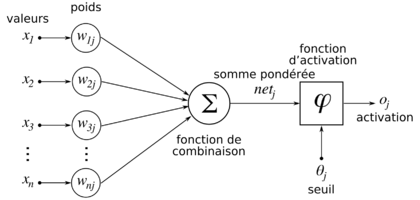
\includegraphics[scale=0.6]{img/neurone.png}}
  \caption{Représentation d'un neurone}
\end{figure}

\noindent Un neurone possède donc une sortie binaire qui découle de la formule suivante :

$$o_{j} = \varphi ((\sum_{i=0}^{n}x_{i} \times w_{i}) - \theta _{j}$$

\noindent La sortie dépend de la fonction et du seuil d'activation qui sont fixés, ainsi que des poids qui composent le neurone. Le réseau de neurones ajuste ces poids durant la phase d'apprentissage afin d'améliorer ses résultats, ce sont donc ces poids que le réseau apprend.\\
 \\
On dit qu'un réseau de neurones est ``profond'' si il est constitué de plusieurs couches de neurones successives (la sortie d'une couche est l'entrée de la suivante): ces réseaux sont souvent plus efficaces sur des problèmes de reconnaissance complexes car les multiples couches leur permettent "d'affiner" successivement ce qui est reconnu (par exemple, pour de la reconnaissance d'images, une première couche pourrait distinguer plusieurs zones de l'image, une seconde les contours des formes qui apparaissent dans ces zones, etc.)

\begin{figure}[h]
  \centerline{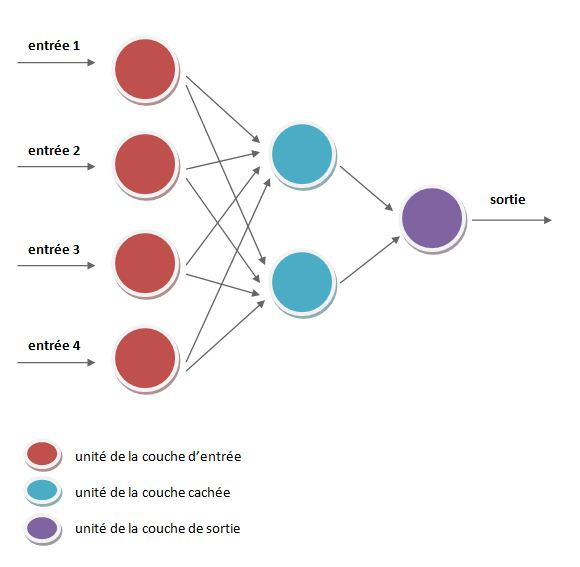
\includegraphics[scale=0.6]{img/organisation_en_couches_rdn.jpg}}
  \caption{Schéma d'un réseau de neurones profond}
\end{figure}

\noindent Le réseau est donc composé de plusieurs couches de neurones qui sont interconnectées.\\  

\subsection{Notre démarche}

L'objectif de ce projet de recherche n'est pas de construire un réseau de neurones par nous-mêmes (nous n'en aurions pas le temps). Pour cette raison, nous allons utiliser une librairie python\footnote{De ce fait, l'intégralité du code que nous allons écrire au cours du projet sera également en python.} qui permet de créer des réseaux de neurones standard de manière très simple et rapide. Notre but sera donc de comprendre comment fonctionne cette librairie, puis de l'utiliser pour construire un (ou plusieurs) réseau qui permettrait de répondre à notre problématique (qui peut donc se résumer par : "Est-il possible d'utiliser un réseau de neurones pour détecter automatiquement la langue d'un contenu audio ?").\\
Les étapes qui suivent résument les différentes parties de notre travail; elles seront détaillées par la suite.\\
 \\
Avant de pouvoir utiliser un réseau de neurones, il est nécessaire de traiter correctement les données dont nous disposons en entrée. Ce prétraitement sera une part importante de notre travail.\\
 \\
\begin{itemize}
  \item Préparation des données (pré-traitement) :
    \begin{dingautolist}{192}
    \item Sélection : Nous avons à disposition un corpus de données audio provenant de sources diverses (émissions de radio, conférences...). Comme tout enregistrement audio, ces fichiers contiennent un certain nombre de passages qui ne sont pas de la parole à proprement dit (musique, applaudissements, silences...), et si ces passages sont trop présents ou trop réguliers, cela risque de biaiser les résultats de notre réseau. Dans un premier temps, nous traiterons donc les fichiers audio afin de supprimer de tels passages.

    \item Paramétrisation : Dans le domaine de la reconnaissance de parole, de manière générale, il est plus efficace de travailler non pas directement avec les signaux audio mais plutôt avec certaines caractéristiques spécifiques extraites de ces signaux. Nous effectuerons donc un traitement acoustique afin d'extraire ces caractéristiques, que l'on mettra en entrée du réseau de neurones.

    \item Stockage : Pour stocker ces ensembles de données, nous utiliserons le format de fichier HDF5, qui permet de classer des groupes de données de manière pratique dans un seul fichier et qui offre certaines options qui nous seront utiles.
    \end{dingautolist}
    
\item Création et utilisation du réseau de neurones
  \begin{dingautolist}{192}
    \addtocounter{enumi}{3}
    \item Formatage des données : Selon son type, un réseau de neurones attend en entrée un ensemble de données organisées de manière spécifique. Nous formaterons donc les données précédemment stockées selon le format d'entrée du réseau utilisé.

    \item Apprentissage et tests : Enfin, il nous restera à créer le réseau proprement dit, puis à réaliser la phase d'apprentissage sur les données formatées. Ensuite , nous pourrons réaliser des tests sur des données nouvelles et affiner les paramètres du réseau pour diminuer son taux d'erreur.
    \end{dingautolist}
  \end{itemize}

\begin{figure}[h]
  \centerline{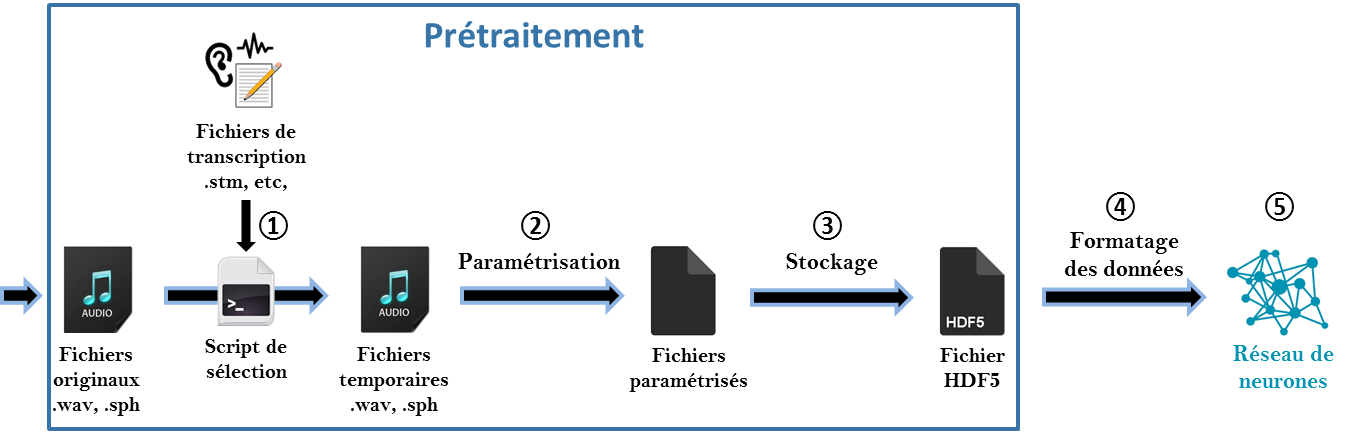
\includegraphics[scale=0.7]{img/schema_complet.png}}
  \caption{Les différentes étapes de notre travail}
\end{figure}
 
\section{Prétraitement : préparation des données}
\hphantom{.}
\begin{figure}[h]
  \centerline{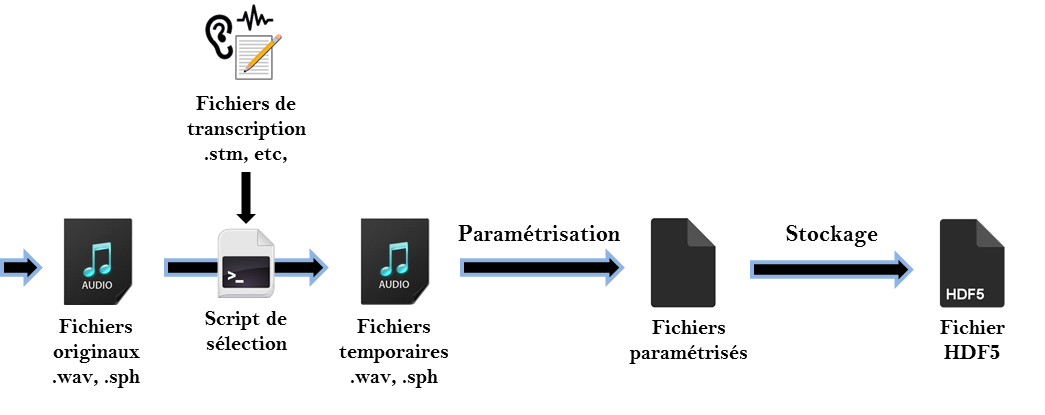
\includegraphics[scale=0.9]{img/schema_pretraitement.png}}
  \caption{Les différentes étapes du prétraitement}
\end{figure}

L'objectif du prétraitement est donc de transformer les données d'entrée (des ensembles de fichiers audio) en un ensemble de données utilisables par le réseau de neurones (des valeurs réelles), stockées sur le disque dur, pour ne pas avoir à refaire le prétraitement à chaque apprentissage du réseau.\\
 \\
 Nous disposons d'un corpus de fichiers de 4 langues différentes (environ une durée totale d'une heure pour chaque) : Arabe, Allemand, Anglais et Français. Les corpus arabe et français sont des extraits d'émissions de radio, le corpus anglais des extraits de conférences, et le corpus allemand des phrases extraites d'un corpus linguistique. En plus des fichiers audio, nous disposons également des fichiers de transcriptions (orthographiques ou phonétiques)\\
*** TRANSCRIPTION ANNEXE ***\\
correspondants qui nous sont utiles pour le prétraitement.

\subsection{Sélection des données utilisables}

\newpage

\hphantom{.}
\begin{figure}[h]
  \centerline{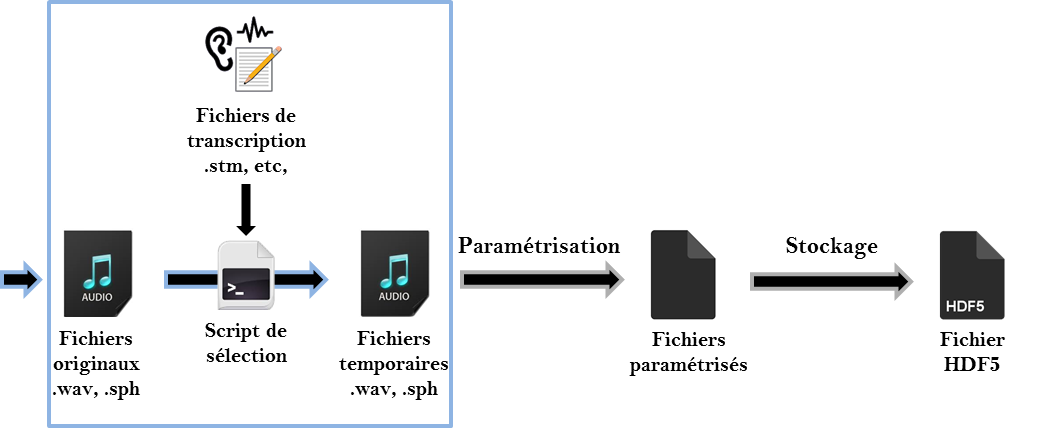
\includegraphics[scale=0.8]{img/schema_selection.png}}
  \caption{La sélection}
\end{figure}

Certains des fichiers audio utilisés peuvent poser problème durant la phase d'apprentissage. En effet, certains commencent ou finissent avec un passage musical ou un silence qui représente une partie non négligeable du fichier. Le problème étant que si un silence ou un passage musical est présent au début ou à la fin dans tous les fichiers audio anglais par exemple, le réseau de neurones risque d'apprendre ce silence ou cette musique comme étant de l'anglais et ainsi de biaiser les résultats sur de futures analyses.\\
\noindent De tels problèmes sont présents sur différents fichiers du corpus dont nous disposons :
\begin{itemize}
    \item les extraits en anglais commencent tous par un morceau musical suivi d'applaudissements ;

    \item les extraits en allemand commencent et se terminent par un silence de durée non négligeable.
    \end{itemize}
    
\noindent Il est donc nécessaire d'enlever ces passages indésirables de manière automatisée. En effet, les retirer à la main aurait demandé beaucoup trop de temps étant donné le grand nombre d'extraits, et il aurait été nécessaire de le refaire pour chaque futur corpus. Pour cela, nous utilisons les transcriptions (orthographiques ou phonétiques) des extraits audio, qui contiennent les temps précis de début et de fin des phrases prononcées.\\
 \\
 Nous avons donc écrit un script afin d'extraire les temps de passage de ``vraie parole'' à l'aide des fichiers de transcription. Pour cela, nous coupons le reste de l'audio des fichiers en utilisant le programme Sox \\
 ***RENVOI VERS SOX***\\(une boîte à outils permettant de faire diverses opérations sur des fichiers audio).

\subsection{Paramétrisation en coefficients acoustiques}

\hphantom{.}
\begin{figure}[h]
  \centerline{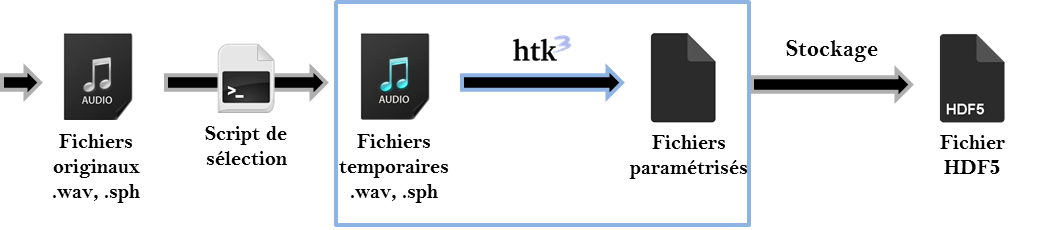
\includegraphics[scale=0.9]{img/schema_parametrisation.png}}
  \caption{La paramétrisation}
\end{figure}
\newpage

Nous pourrions utiliser directement les signaux audio en entrée de notre réseau de neurones : il nous suffirait par exemple de relever la valeur du signal tous les X intervalles de temps et de fournir directement ces valeurs au réseau. Cependant, dans le domaine de la reconnaissance de parole, on utilise plutôt des signaux paramétrisés.
La paramétrisation d'un signal consiste en l'extraction d'un ensemble spécifique de caractéristiques de ce signal. \\
\\
*** A PRECISEEEEEER ***\\
Pour effectuer cette paramétrisation, nous utilisons HTK\\
 ***RENVOI VERS HTK***\\, un logiciel multiplateforme développé par le département d'ingénierie de l'Université de Cambridge, qui est une sorte de ``boîte à outils'' permettant de réaliser toutes sortes de manipulations utiles à la reconnaissance de la parole. Il permet notamment d'effectuer de manière très simple la paramétrisation de fichiers audio en coefficients acoustiques correspondants. Les fichiers ainsi obtenus sont des fichiers .mfcc (Mel-frequency cepstral coefficients).
 
\subsection{Stockage des données}

\hphantom{.}
\begin{figure}[h]
  \centerline{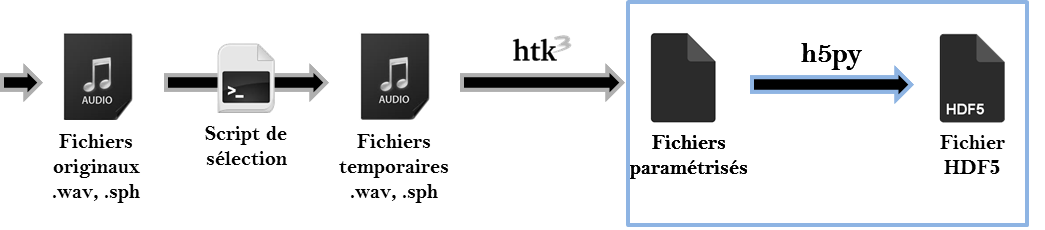
\includegraphics[scale=0.9]{img/schema_stockage.png}}
  \caption{Le stockage des données}
\end{figure}

Afin de ne pas répéter la phase de prétraitement à chaque apprentissage du réseau de neurones, il est primordial de stocker les données pré-traitées. Pour cela, nous utilisons le format de données HDF5\\ ***RENVOI VERS HDF5***\\ (grâce à la bibliothèque python h5py) qui nous permet de hiérarchiser et d'organiser facilement nos données une fois le prétraitement terminé.\\
 \\
 Ce format possède également un autre avantage qui nous est très utile : il permet si nécessaire de transmettre des données en les chargeant directement depuis le disque dur. En effet, pour éviter les régularités dans les fichiers de données qui pourraient biaiser le processus d'apprentissage, les données en entrée du réseau de neurones seront mélangées avant le début de l'apprentissage. Pour ce faire, il est nécessaire de lui fournir l'intégralité des données en une seule fois. De ce fait, la quantité de données générée par la transformation des fichiers audio en coefficients acoustiques peut être trop importante pour pouvoir charger les données directement en mémoire vive selon la taille de départ du corpus. Le format de données HDF5 nous permet donc de parer à ce problème éventuel en chargeant les données directement depuis le disque dur sans surcharger la mémoire vive, même si la vitesse de traitement s'en trouve diminuée.\\
 \\
Au final, la taille des données ne nous a pas posé de problème, étant suffisamment petite pour être chargée en mémoire. Néanmoins, nous avons quand même écrit une fonction qui utilise cette caractéristique du format HDF5, qui pourrait être utile dans le futur, si on a un jour besoin de traiter plus de données.

\section{Utilisation des réseaux de neurones}

\hphantom{.}
\begin{figure}[h]
  \centerline{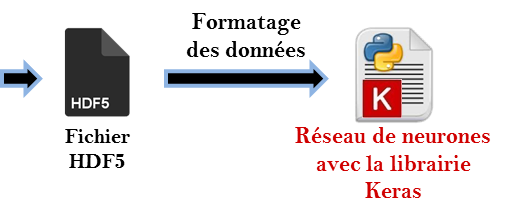
\includegraphics[scale=0.9]{img/schema_reseau_keras.png}}
  \caption{L'utilisation du réseau de neurones}
\end{figure}

Une fois les données mises en bonne forme dans notre fichier HDF5, nous pouvons les transmettre au réseau de neurones et de commencer l'apprentissage. Pour cela, il nous faudra formater les données sous la forme attendue par le réseau (qui pourra changer selon le type de réseau construit) et trouver les bons paramètres pour le réseau qui nous permettront d'obtenir de meilleurs taux de reconnaissance.

\subsection{Keras}

Keras est une librairie open-source Python utilisée pour construire, entraîner et manipuler des réseaux de neurones artificiels, développée par François Chollet dans le cadre du projet de recherche ONEIROS (Open-ended Neuro-Electronic Intelligent Robot Operating System). L'avantage de cette librairie est qu'elle est très haut niveau, elle permet donc de créer des réseaux de neurones très rapidement et très simplement. En effet, cette dernière n'est en quelque sorte qu'une "interface de surcouche" qui se place au-dessus de librairies de réseaux de neurones plus bas niveau comme Theano, qui est la sous-couche que nous utiliserons avec Keras.\\
 \\
Il est possible de créer un réseau de neurones (parfois complexe) avec Keras en littéralement quelques lignes :\\

\pythonexternal[showstringspaces=false, breaklines=true,breakatwhitespace=true]{exempleReseau.py}

De plus, Keras est très pratique à utiliser en python (les réseaux créés fonctionnant avec des tableaux numpy classiques\footnote{Numpy est une bibliothèque scientifique très utilisée en Python, qui offre notamment la possibilité de réaliser simplement des calculs matriciels.}) et dispose de beaucoup d'options, qui permettent par exemple d'interrompre l'apprentissage dès qu'on le juge nécessaire, de sauvegarder un modèle de réseau, d'optimiser la lecture depuis un fichier HDF5...

\subsection{Définir l'architecture du réseau}

*** Renvoi biblio vers l'article Y.LeCun***

\subsubsection{Généralités sur la création de réseaux de neurones}
Lorsque on crée un réseau de neurones, il est nécessaire d'en définir la structure. Le premier paramètre de cette structure est le nombre de couches du réseau. Ajouter plus de couches permet d'apprendre des paramètres plus ``précis'' sur les données. Ce qui n'est pas forcément une bonne chose si ces paramètres représentent moins bien la caractéristique des entrées que l'on cherche à déterminer (la langue dans notre cas).\\
 \\
Il nous faut aussi déterminer la taille de ces couches (le nombre de neurones qu'elles contiennent). La taille de la couche d'entrée doit être la même que le nombre de valeurs contenues dans un exemple du corpus d'apprentissage, et la taille de la couche de sortie dépend du nombre de langues différentes qu'on souhaite détecter. La taille des couches cachées est quand à elle habituellement comprise entre celle de la couche d'entrée et celle de la couche de sortie; c'est un des paramètres que l'on peut ajuster pour améliorer la performance du réseau.\\
 \\
Chacune de ces couches comporte une fonction d'activation (qui sera appliquée à chacun des neurones de la couche). Cette fonction régit la sortie du neurone en comparant la somme des poids à un seuil. Il existe différents types de fonctions d'activation, qui peuvent se comporter de manière différente : on utilise souvent une fonction différente de celle des autres couches pour la couche de sortie, par exemple.\\
 \\
Enfin, il existe différents types de réseaux de neurones, qui ont un fonctionnement interne différent.  Pour ce projet, nous en avons considéré deux : un perceptron multi-couches et un réseau LSTM (Long Short-Term Memory).
 
\subsubsection{Perceptron multi-couches}

Le perceptron multi-couches est un des modèles de réseau les plus simples à mettre en œuvre mais qui peut donner de très bons résultats. C'est historiquement un des tout premiers modèles d'apprentissage supervisé. Il est ``simplement'' constitué de plusieurs couches de neurones, la sortie des neurones d'une couche constituant l'entrée des neurones de la couche suivante.\\
 \\
Pour ce perceptron multi-couches, nous utilisons deux couches de taille (nombre de valeurs dans un vecteur acoustique $\times$ nombre de vecteurs dans une trame) dont la couche d'entrée, pour avoir effectivement un neurone par valeur réelle, et une couche de sortie de taille 4, puisque nous avons 4 langages possibles différents. Entre les deux, nous avons deux couches cachées, dont nous avons fixé la taille à 256 (suivant les instructions de nos encadrants).\\
La fonction d'activation des couches d'entrée et des couches cachées est une fonction ReLU (Rectified Linear Unit) : il s'agit plus ou moins de la fonction la plus efficace, de manière générale, pour le moment pour cette application précise. Elle peut être approximée par :
$$ f(x) = ln(1 + e^{x}) $$
La fonction d'activation de la couche de sortie est une fonction softmax : c'est à dire que, pour chaque entrée, le réseau générera 4 probabilités dont la somme est égale à 1 : la probabilité que l'entrée soit du français, la probabilité que l'entrée soit de l'allemand... et donnera en sortie la langue dont la probabilité est la plus élevée.\\

*** Code commenté de la création du perceptron ***

\subsubsection{Réseau LSTM (Long Short-Term Memory)}

Les réseaux LSTM sont des réseaux récurrents. Le principe d'un réseau récurrent est de se ``souvenir'' des résultats de l'apprentissage de données précédentes pour essayer d'améliorer sa performance sur les données actuelles :autrement dit, en utilisant les résultats des prédictions sur les données précédentes lors de l'évaluation des données actuelles, on utilise un contexte qui peut aider à prendre une décision.\\
 \\
Le nombre de couches, les fonctions d'activation et la taile des couches cachées et de sortie de ce réseau sont les mêmes que celles du perceptron multi-couches. La taille de la couche d'entrée va différer : en effet, pour pouvoir fournir un contexte pertinent lors de l'évaluation suivante, on a besoin de retenir plus qu'une seule trame de données. On ne va donc plus fournir en entrée du réseau une seule trame mais un ensemble de trames (de taille fixe); le résultat de l'évaluation d'un ensemble de trames aura donc de l'influence sur l'évaluation de l'ensemble de trames suivant.\\
 \\
Néanmoins, par manque de temps lors de la fin du projet, nous n'avons pas pu implémenter ce type de réseau.

\subsection{Apprendre les paramètres du réseau sur le corpus d'apprentissage}

\subsubsection{Généralités sur les mécanismes d'apprentissage}

Pour faire l'apprentissage proprement dit, le réseau va procéder de la manière suivante :
\begin{itemize}
  \item Prendre une certaine quantité (fixe) X de données parmi l'ensemble d'apprentissage qu'il a reçu, de manière aléatoire,
  \item Passer ces données X à travers les différentes couches du réseau,
  \item Obtenir le résultat de la prédiction à la couche de sortie, puis le comparer à l'étiquette de X et réajuster les différentes couches par rapport à ce résultat,
  \item Répéter jusqu'à avoir traité toutes les données de l'ensemble d'apprentissage.
\end{itemize}

\hphantom{.}
\begin{figure}[h]
  \centerline{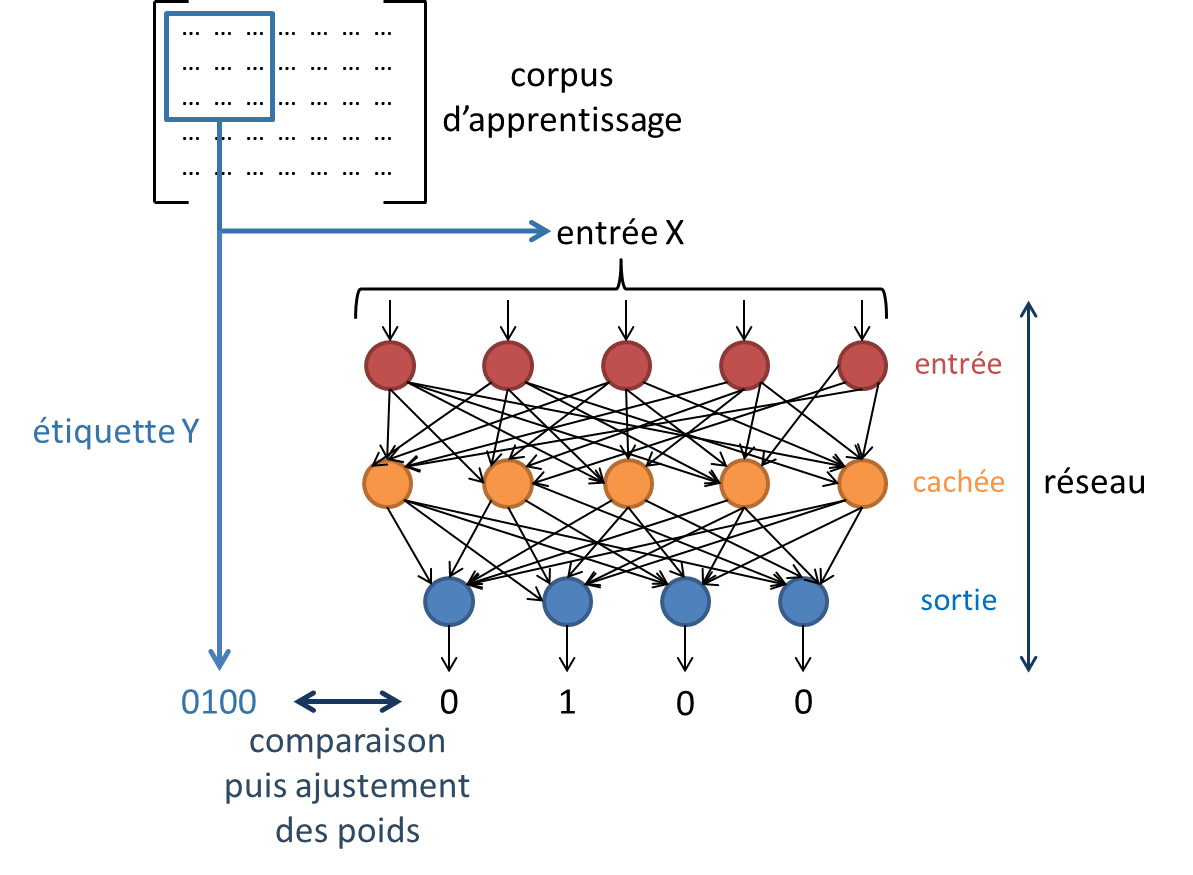
\includegraphics[scale=0.6]{img/schema_epoch.png}}
  \caption{Représentation d'une epoch d'apprentissage}
\end{figure}

\noindent Ce traitement de toutes les données du corpus d'apprentissage s'appelle une epoch. On effectue généralement plusieurs epochs pour un apprentissage (pour nous, environ une centaine), les performances du réseau étant censées s'améliorer au fil des epochs. \\
 \\
Pour améliorer les capacités d'apprentissage de notre réseau, nous utilisons une méthode classique d'apprentissage automatique qui consiste à séparer nos données d'apprentissage en 2 corpus distincts : 

\begin{itemize}
\item un corpus d'apprentissage (appelé train), qu'on va envoyer en entrée du réseau de neurones et qui sera directement ``appris'',
\item et un corpus de validation (appelé dev), sur lequel le réseau va tester ses capacités après chaque epoch, et utiliser les résultats de ce test pour améliorer l'apprentissage sur le corpus de base.
\end{itemize}

\noindent inalement, si l'apprentissage se déroule conformément à ce qu'on attendait, on utilise le corpus de test pour évaluer les performances de notre modèle sur des données qu'il n'a jamais vues.
\newpage
\subsubsection{Formatage des données pour le perceptron multi-couches}

En entrée du réseau, nous ne pouvons pas simplement mettre un seul vecteur acoustique à la fois : en effet, cela n'a pas vraiment de sens d'essayer d'en prédire la langue puisqu'il correspond à une durée de parole très courte, de quelques millisecondes seulement. Pour cette raison, nous passons en entrée un ensemble de ces vecteurs, que l'on appelle une trame, et dont la durée de parole combinée correspondant aux vecteurs qui la compose fait plutôt quelques dizaines de millisecondes, ce qui peut permettre de plutôt travailler sur des syllabes ou des mots courts. Le nombre de vecteurs composant cette trame est donc un des paramètres de notre réseau.\\
 \\
De plus, afin d'être sûrs de repérer tous les ``traits'' de caractère possibles d'un langage, nous utilisons une fenêtre glissante (fig. 11) : plutôt que de séparer un fichier d'entrée en le découpant en X trames successives, nous ``décalons'' chaque trame successive d'un certain nombre de vecteurs; ainsi, nous obtenons un ensemble de trames où les $n$ premiers vecteurs de l'une sont les $n$ derniers vecteurs de la précédente. Ce décalage est donc aussi un paramètre de notre réseau.

\hphantom{.}
\begin{figure}[h]
  \centerline{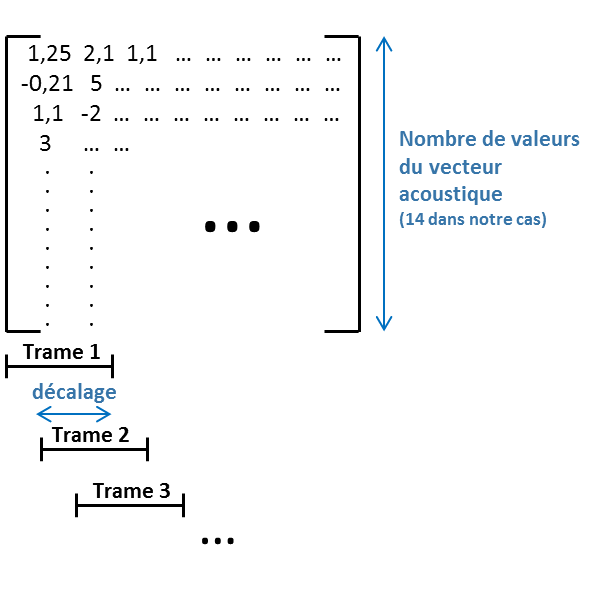
\includegraphics[scale=0.8]{img/schema_decoupage_trame.png}}
  \caption{Découpage des données en trames}
\end{figure}

\subsubsection{Résultat de l'apprentissage sur le perceptron multi-couches}

Le premier apprentissage que nous avons effectué sur le perceptron s'est révélé infructueux. En effet, le réseau apprenait correctement sur le corpus d'apprentissage et s'améliorait linéairement au fur et à mesure mais ne s'améliorait pas sur le corpus de validation et stagnait aux alentours de 50\% de précision, ce qui semblait indiquer que le réseau n'apprenait rien d'assez général qui puisse l'aider à s'améliorer sur le corpus de validation.\\
 \\
Nous avons ensuite effectué d'autres apprentissages en faisant varier les différents paramètres (taille des trames d'entrée, décalage), notamment en augmentant la taille des trames d'entrée de manière significative sur certains essais en partant de la supposition que la taille des trames était peut-être insuffisante pour apporter de l'information pertinente au réseau.\\
\noindent Nous avons également essayé de normaliser les données en mettant la variance de chaque composante des vecteurs acoustiques à 1 pour les corpus d'apprentissage et de validation).\\
\noindent Tous les essais sur le perceptron ont cependant conduit au même résultat que précédemment : aucune amélioration sur le corpus de validation pendant la phase d'apprentissage.

\subsection{Utiliser le réseau pour étiqueter le corpus de test}

Une fois que le réseau est créé et entraîné, nous pouvons l'utiliser pour prédire la langue de fichiers audio qui ne sont pas étiquetés. Pour ce faire, nous appliquons aux fichiers de test le même traitement qu'aux fichiers d'apprentissage : paramétrisation en coefficients acoustiques, stockage dans un fichier HDF5, etc. Mais, à la différence des données d'apprentissage, ces données là ne sont pas étiquetées : on ne fournit pas au réseau la langue parlée. Il suffit ensuite simplement de mettre ces données en entrée du réseau de neurones et d'observer l'état de la couche de sortie pour savoir quelle langue a prédit notre réseau pour ce fichier.\\
 \\
Les résultats des tests du perceptron multi-couches sur un ensemble de fichiers de test nous ont confirmé que le réseau n'est effectivement pas efficace : il ne parvient à prédire correctement que peu de fichiers, et se comporte de manière étrange sur certains passages. La raison de cette inefficacité est probablement qu'un réseau aussi simple n'est pas assez puissant pour détecter suffisement des paramètres pour pouvoir classifier correctement les langues.\\ *** Renvoi en annexe à des résultats de tests expliqués ***\\

\section{Conclusion}

\bibliographystyle{plain}
\bibliography{biblio}

\end{document}
